\documentclass[11pt,a4paper]{article}
\usepackage[polish]{fga}
\usepackage{icomma}
\usepackage{placeins}
\DeclareMathOperator{\artanh}{artanh}
% Generated by python -m src.problems. Do not edit.
\newcommand{\gcShorter}{17}
\newcommand{\gcLonger}{3}
\newcommand{\gcEqual}{0}
\newcommand{\gcMedian}{0{,}75}
\newcommand{\gcRatioMin}{0{,}16}
\newcommand{\gcRatioMax}{1{,}92}
\newcommand{\gcSumClassic}{1098}
\newcommand{\gcSumNew}{752}
\newcommand{\gcResidMax}{7{,}2\cdot10^{-12}}
\newcommand{\gcTight}{17}
\newcommand{\gcRatioMinId}{H}
\newcommand{\gcRatioMaxId}{C}
\newcommand{\gcLongerIds}{C, D, J}
\newcommand{\gcClassicA}{\theta = \arccos\frac{I_3\omega_3}{L} \\ \varphi(t) = \frac{L}{I_1}\,t \\ \psi(t) = \frac{I_1 - I_3}{I_1}\,\omega_3 t \\ \mathsf{R}(t) = \mathsf{R}_z(\varphi)\,\mathsf{R}_x(\theta)\,\mathsf{R}_z(\psi)}
\newcommand{\gcNewA}{R(t) = \exp\left(-\frac{t}{2I_1}\,\mathcal{I}\mathbf{L}\right) R_0\, \exp\left(-\frac{t}{2}\,\Omega\,\mathcal{I}e_3\right) \\ \Omega = \frac{I_1 - I_3}{I_1}\,\omega_3}
\newcommand{\gcLenClassicA}{55}
\newcommand{\gcLenNewA}{41}
\newcommand{\gcResidA}{2{,}9\cdot10^{-12}}
\newcommand{\gcClassicB}{V'(r) = 4\epsilon\left(-\frac{12\sigma^{12}}{r^{13}} + \frac{6\sigma^{6}}{r^{7}}\right) \\ V''(r) = 4\epsilon\left(\frac{156\sigma^{12}}{r^{14}} - \frac{42\sigma^{6}}{r^{8}}\right) \\ V'(r_0) = 0, \quad \omega = \sqrt{\frac{V''(r_0)}{m}}}
\newcommand{\gcNewB}{V(r_0 + \varepsilon) = V_0 + c_1\varepsilon + c_2\varepsilon^2, \quad \varepsilon^3 = 0 \\ c_1 = 0, \quad \omega = \sqrt{\frac{2c_2}{m}}}
\newcommand{\gcLenClassicB}{77}
\newcommand{\gcLenNewB}{39}
\newcommand{\gcResidB}{1{,}8\cdot10^{-15}}
\newcommand{\gcLJk}{57{,}146}
\newcommand{\gcLJomega}{7{,}560}
\newcommand{\gcLJfd}{8{,}8\cdot10^{-10}}
\newcommand{\gcClassicC}{M = \sqrt{\frac{\mu}{a^3}}\,t \\ M = E - e\sin E \\ x = a(\cos E - e) \\ y = a\sqrt{1 - e^2}\,\sin E}
\newcommand{\gcNewC}{z = w^2, \quad \frac{d^2w}{ds^2} = -\omega^2 w, \quad \omega = \frac{1}{2}\sqrt{\frac{\mu}{a}} \\ w = \sqrt{a(1-e)}\cos\omega s + i\sqrt{a(1+e)}\sin\omega s \\ t = as - \frac{ae}{2\omega}\sin 2\omega s}
\newcommand{\gcLenClassicC}{36}
\newcommand{\gcLenNewC}{69}
\newcommand{\gcResidC}{1{,}4\cdot10^{-14}}
\newcommand{\gcKeplerOrders}{10}
\newcommand{\gcClassicD}{v_\infty = \sqrt{(v_p + \Delta v)^2 - \frac{2\mu}{r_p}}}
\newcommand{\gcNewD}{v_\infty = (v_p + \Delta v) \ominus v_e, \quad v_e = \sqrt{\frac{2\mu}{r_p}}, \quad g(v) = v^2}
\newcommand{\gcLenClassicD}{19}
\newcommand{\gcLenNewD}{32}
\newcommand{\gcResidD}{9{,}8\cdot10^{-14}}
\newcommand{\gcOberth}{0{,}458}
\newcommand{\gcClassicE}{x = e^{-\gamma t}\left(x_0\cos\Omega t + \frac{v_0 + \gamma x_0}{\Omega}\sin\Omega t\right), \quad \gamma < \omega_0 \\ x = e^{-\gamma t}\left(x_0 + (v_0 + \gamma x_0)\,t\right), \quad \gamma = \omega_0 \\ x = e^{-\gamma t}\left(x_0\cosh\Omega t + \frac{v_0 + \gamma x_0}{\Omega}\sinh\Omega t\right), \quad \gamma > \omega_0 \\ \Omega = \sqrt{|\omega_0^2 - \gamma^2|}}
\newcommand{\gcNewE}{x = e^{-\gamma t}\left(x_0 C + (v_0 + \gamma x_0) S\right) \\ C + \mathbf{e}S = \exp(\mathbf{e}t), \quad \mathbf{e}^2 = \gamma^2 - \omega_0^2}
\newcommand{\gcLenClassicE}{101}
\newcommand{\gcLenNewE}{45}
\newcommand{\gcResidE}{5{,}7\cdot10^{-15}}
\newcommand{\gcClassicF}{L = 10\log_{10}\left(10^{L_1/10} + 10^{L_2/10}\right)}
\newcommand{\gcNewF}{L = L_1 \oplus_h L_2, \quad h = \frac{10}{\ln 10}}
\newcommand{\gcLenClassicF}{20}
\newcommand{\gcLenNewF}{15}
\newcommand{\gcResidF}{1{,}4\cdot10^{-14}}
\newcommand{\gcDbSame}{83{,}01}
\newcommand{\gcDbTen}{0{,}41}
\newcommand{\gcDbH}{4{,}34}
\newcommand{\gcClassicG}{Z = e^{-Nf_1/T} + e^{-Nf_2/T} \\ f = -\frac{T}{N}\ln Z \\ \lim_{N\to\infty} f = \min(f_1, f_2)}
\newcommand{\gcNewG}{f = f_1 \oplus_h f_2, \quad h = -\frac{T}{N} \\ \lim_{h\to 0^-} f = \min(f_1, f_2)}
\newcommand{\gcLenClassicG}{41}
\newcommand{\gcLenNewG}{31}
\newcommand{\gcResidG}{5{,}6\cdot10^{-17}}
\newcommand{\gcSchottkyT}{0{,}417}
\newcommand{\gcSchottkyC}{0{,}439}
\newcommand{\gcClassicH}{\left(\frac{\partial T}{\partial V}\right)_S = -\left(\frac{\partial p}{\partial S}\right)_V \\ \left(\frac{\partial T}{\partial p}\right)_S = \left(\frac{\partial V}{\partial S}\right)_p \\ \left(\frac{\partial S}{\partial V}\right)_T = \left(\frac{\partial p}{\partial T}\right)_V \\ \left(\frac{\partial S}{\partial p}\right)_T = -\left(\frac{\partial V}{\partial T}\right)_p}
\newcommand{\gcNewH}{dT \wedge dS = dp \wedge dV}
\newcommand{\gcLenClassicH}{70}
\newcommand{\gcLenNewH}{11}
\newcommand{\gcResidH}{2{,}3\cdot10^{-8}}
\newcommand{\gcCarnotArea}{0{,}6931}
\newcommand{\gcClassicI}{\nabla\cdot\mathbf{E} = \frac{\rho}{\varepsilon_0} \\ \nabla\cdot\mathbf{B} = 0 \\ \nabla\times\mathbf{E} = -\frac{\partial\mathbf{B}}{\partial t} \\ \nabla\times\mathbf{B} = \mu_0\mathbf{J} + \frac{1}{c^2}\frac{\partial\mathbf{E}}{\partial t}}
\newcommand{\gcNewI}{\left(\frac{1}{c}\frac{\partial}{\partial t} + \nabla\right)F = \frac{\rho}{\varepsilon_0} - c\mu_0\mathbf{J}, \quad F = \mathbf{E} + \mathcal{I}c\mathbf{B}}
\newcommand{\gcLenClassicI}{41}
\newcommand{\gcLenNewI}{30}
\newcommand{\gcResidI}{4{,}4\cdot10^{-16}}
\newcommand{\gcClassicJ}{Z_i = Z_0\,\frac{Z_L + jZ_0\tan\beta l}{Z_0 + jZ_L\tan\beta l}}
\newcommand{\gcNewJ}{g(z_i) = g(z_L) + j\beta l, \quad g = \artanh, \quad z = \frac{Z}{Z_0}}
\newcommand{\gcLenClassicJ}{24}
\newcommand{\gcLenNewJ}{26}
\newcommand{\gcResidJ}{1{,}0\cdot10^{-14}}
\newcommand{\gcClassicK}{n_1\sin\theta_1 = n_2\sin\theta_2 \\ \sin\theta_1 = \frac{x}{\sqrt{a^2 + x^2}}, \quad \sin\theta_2 = \frac{d - x}{\sqrt{b^2 + (d - x)^2}} \\ T = \frac{n_1}{c}\sqrt{a^2 + x^2} + \frac{n_2}{c}\sqrt{b^2 + (d - x)^2}}
\newcommand{\gcNewK}{T = \bigoplus_x \left(T_1(x) + T_2(x)\right), \quad \oplus = \min \\ T_1 = \frac{n_1}{c}\sqrt{a^2 + x^2}, \quad T_2 = \frac{n_2}{c}\sqrt{b^2 + (d - x)^2}}
\newcommand{\gcLenClassicK}{77}
\newcommand{\gcLenNewK}{60}
\newcommand{\gcResidK}{7{,}2\cdot10^{-12}}
\newcommand{\gcSnellDefect}{4{,}5\cdot10^{-6}}
\newcommand{\gcClassicL}{I = I_0\left(\sum_{k=0}^{N-1}\cos k\delta\right)^2 + I_0\left(\sum_{k=0}^{N-1}\sin k\delta\right)^2 \\ \sum_{k=0}^{N-1}\cos k\delta = \frac{\sin\frac{N\delta}{2}}{\sin\frac{\delta}{2}}\cos\frac{(N-1)\delta}{2} \\ \sum_{k=0}^{N-1}\sin k\delta = \frac{\sin\frac{N\delta}{2}}{\sin\frac{\delta}{2}}\sin\frac{(N-1)\delta}{2}}
\newcommand{\gcNewL}{I = I_0\left|\sum_{k=0}^{N-1} q^k\right|^2 = I_0\left|\frac{1 - q^N}{1 - q}\right|^2, \quad q = \exp(i\delta)}
\newcommand{\gcLenClassicL}{99}
\newcommand{\gcLenNewL}{43}
\newcommand{\gcResidL}{7{,}1\cdot10^{-16}}
\newcommand{\gcClassicM}{\tan\frac{\theta}{2} = \frac{\sin\alpha}{D + \cos\alpha}, \quad D = \sqrt{\frac{(\gamma_1 + 1)(\gamma_2 + 1)}{(\gamma_1 - 1)(\gamma_2 - 1)}}}
\newcommand{\gcNewM}{R\,B = \exp\left(\frac{\eta_2}{2}\mathbf{n}_2\right)\exp\left(\frac{\eta_1}{2}\mathbf{n}_1\right) \\ \theta \approx \frac{1}{2}\eta_1\eta_2\sin\alpha}
\newcommand{\gcLenClassicM}{41}
\newcommand{\gcLenNewM}{32}
\newcommand{\gcResidM}{1{,}2\cdot10^{-14}}
\newcommand{\gcWignerDeg}{42{,}9}
\newcommand{\gcWignerSmall}{0{,}998}
\newcommand{\gcClassicN}{\frac{d^2u}{d\varphi^2} + u = \frac{\mu}{h^2} + \frac{3\mu}{c^2}u^2 \\ u \approx \frac{\mu}{h^2}\left(1 + e\cos\varphi + \lambda e\varphi\sin\varphi\right) \\ u \approx \frac{\mu}{h^2}\left(1 + e\cos((1 - \lambda)\varphi)\right) \\ \Delta\varphi = 2\pi\lambda, \quad \lambda = \frac{3\mu^2}{c^2h^2}}
\newcommand{\gcNewN}{u_0 = 1 + \lambda u_0^2, \quad \Omega^2 = 1 - 2\lambda u_0, \quad \lambda^2 = 0 \\ \Delta\varphi = 2\pi\left(\frac{1}{\Omega} - 1\right) = 2\pi\lambda, \quad \lambda = \frac{3\mu^2}{c^2h^2}}
\newcommand{\gcLenClassicN}{88}
\newcommand{\gcLenNewN}{57}
\newcommand{\gcResidN}{2{,}5\cdot10^{-5}}
\newcommand{\gcMercuryArcsec}{42{,}98}
\newcommand{\gcMercuryLambda}{7{,}99}
\newcommand{\gcClassicO}{i\hbar\frac{d\psi}{dt} = \frac{\hbar}{2}\begin{pmatrix}\Delta & \Omega_R \\ \Omega_R & -\Delta\end{pmatrix}\psi \\ P = \frac{\Omega_R^2}{\Omega_R^2 + \Delta^2}\sin^2\frac{\sqrt{\Omega_R^2 + \Delta^2}\,t}{2}}
\newcommand{\gcNewO}{\mathbf{s}(t) = R\,e_3\,\tilde{R}, \quad R = \exp\left(-\frac{t}{2}\,\mathcal{I}(\Omega_R e_1 + \Delta e_3)\right) \\ P = \frac{1 - \mathbf{s}\cdot e_3}{2}}
\newcommand{\gcLenClassicO}{50}
\newcommand{\gcLenNewO}{41}
\newcommand{\gcResidO}{3{,}7\cdot10^{-12}}
\newcommand{\gcClassicP}{\frac{d}{dt}\frac{\partial L}{\partial\dot{x}} - \frac{\partial L}{\partial x} = 0 \\ S = \int_0^T L\,dt = \frac{mX^2}{2T}}
\newcommand{\gcNewP}{S = \lim_{\hbar\to 0}\,\bigoplus_{x} S(x), \quad \oplus = \oplus_h, \quad h = -i\hbar}
\newcommand{\gcLenClassicP}{35}
\newcommand{\gcLenNewP}{27}
\newcommand{\gcResidP}{4{,}3\cdot10^{-4}}
\newcommand{\gcClassicQ}{\lambda = \frac{\ln 2}{T_1} + \frac{\ln 2}{T_2} \\ T = \frac{\ln 2}{\lambda} = \frac{T_1T_2}{T_1 + T_2}}
\newcommand{\gcNewQ}{T = T_1 \oplus T_2, \quad g(x) = \frac{1}{x}}
\newcommand{\gcLenClassicQ}{30}
\newcommand{\gcLenNewQ}{16}
\newcommand{\gcResidQ}{2{,}2\cdot10^{-16}}
\newcommand{\gcHalfEff}{7{,}27}
\newcommand{\gcClassicR}{E + mc^2 = E' + \sqrt{p^2c^2 + m^2c^4} \\ \frac{E}{c} = \frac{E'}{c}\cos\theta + p\cos\phi \\ 0 = \frac{E'}{c}\sin\theta - p\sin\phi \\ \frac{1}{E'} = \frac{1}{E} + \frac{1 - \cos\theta}{mc^2}}
\newcommand{\gcNewR}{(p + k - k')^2 = m^2c^2 \\ E' = E \oplus \frac{mc^2}{1 - \cos\theta}, \quad g(x) = \frac{1}{x}}
\newcommand{\gcLenClassicR}{68}
\newcommand{\gcLenNewR}{40}
\newcommand{\gcResidR}{9{,}9\cdot10^{-15}}
\newcommand{\gcClassicS}{m\ddot{u}_n = K(u_{n+1} - 2u_n + u_{n-1}) \\ u_n = A\exp(i(kna - \omega t)), \quad u_{n+N} = u_n \\ \omega_k = 2\sqrt{\frac{K}{m}}\left|\sin\frac{\pi k}{N}\right|}
\newcommand{\gcNewS}{D = \frac{K}{m}\left(2 - s - s^{-1}\right), \quad s^N = 1 \\ \omega_k^2 = D\left(s = \exp\frac{2\pi ik}{N}\right) = \frac{4K}{m}\sin^2\frac{\pi k}{N}}
\newcommand{\gcLenClassicS}{60}
\newcommand{\gcLenNewS}{50}
\newcommand{\gcResidS}{2{,}2\cdot10^{-15}}
\newcommand{\gcClassicT}{\phi = U\left(r + \frac{a^2}{r}\right)\cos\theta - \frac{\Gamma}{2\pi}\theta \\ p = p_\infty + \frac{\rho}{2}\left(U^2 - \left(2U\sin\theta + \frac{\Gamma}{2\pi a}\right)^2\right) \\ Y = -\int_0^{2\pi} p\sin\theta\,a\,d\theta = \rho U\Gamma}
\newcommand{\gcNewT}{w = U\left(z + \frac{a^2}{z}\right) + \frac{i\Gamma}{2\pi}\ln z \\ X - iY = \frac{i\rho}{2}\oint\left(\frac{dw}{dz}\right)^2 dz = -i\rho U\Gamma}
\newcommand{\gcLenClassicT}{66}
\newcommand{\gcLenNewT}{47}
\newcommand{\gcResidT}{8{,}9\cdot10^{-16}}
\newcommand{\gcRows}{%
A & Swobodny bąk symetryczny & jednostka & 55 & 41 & $0{,}75$ & $2{,}9\cdot10^{-12}$ \\
B & Częstość drgań wokół minimum & jednostka & 77 & 39 & $0{,}51$ & $1{,}8\cdot10^{-15}$ \\
C & Orbita Keplera & jednostka & 36 & 69 & $1{,}92$ & $1{,}4\cdot10^{-14}$ \\
D & Nadwyżka hiperboliczna & skala & 19 & 32 & $1{,}68$ & $9{,}8\cdot10^{-14}$ \\
E & Oscylator tłumiony & jednostka & 101 & 45 & $0{,}45$ & $5{,}7\cdot10^{-15}$ \\
F & Suma poziomów dźwięku & temperatura & 20 & 15 & $0{,}75$ & $1{,}4\cdot10^{-14}$ \\
G & Energia swobodna dwóch faz & temperatura & 41 & 31 & $0{,}76$ & $5{,}6\cdot10^{-17}$ \\
H & Relacje Maxwella & jednostka & 70 & 11 & $0{,}16$ & $2{,}3\cdot10^{-8}$ \\
I & Równania Maxwella & jednostka & 41 & 30 & $0{,}73$ & $4{,}4\cdot10^{-16}$ \\
J & Impedancja wejściowa linii & skala & 24 & 26 & $1{,}08$ & $1{,}0\cdot10^{-14}$ \\
K & Załamanie światła & temperatura & 77 & 60 & $0{,}78$ & $7{,}2\cdot10^{-12}$ \\
L & Dyfrakcja na N szczelinach & jednostka & 99 & 43 & $0{,}43$ & $7{,}1\cdot10^{-16}$ \\
M & Obrót Thomasa--Wignera & komutator & 41 & 32 & $0{,}78$ & $1{,}2\cdot10^{-14}$ \\
N & Peryhelium Merkurego & jednostka & 88 & 57 & $0{,}65$ & $2{,}5\cdot10^{-5}$ \\
O & Oscylacje Rabiego spinu & jednostka & 50 & 41 & $0{,}82$ & $3{,}7\cdot10^{-12}$ \\
P & Najmniejsze działanie & temperatura & 35 & 27 & $0{,}77$ & $4{,}3\cdot10^{-4}$ \\
Q & Efektywny okres półtrwania & skala & 30 & 16 & $0{,}53$ & $2{,}2\cdot10^{-16}$ \\
R & Rozpraszanie Comptona & jednostka & 68 & 40 & $0{,}59$ & $9{,}9\cdot10^{-15}$ \\
S & Fonony w łańcuchu atomów & jednostka & 60 & 50 & $0{,}83$ & $2{,}2\cdot10^{-15}$ \\
T & Opływ walca z cyrkulacją & jednostka & 66 & 47 & $0{,}71$ & $8{,}9\cdot10^{-16}$ \\
}

\renewcommand{\topfraction}{0.9}
\renewcommand{\textfraction}{0.08}
\renewcommand{\floatpagefraction}{0.85}

% notation of this paper
\newcommand{\ue}{\mathbf{e}}                 % a unit
\newcommand{\ps}{\mathcal{I}}                % the product e_1 e_2 e_3
\newcommand{\oph}{\mathbin{\oplus_{h}}}       % thermal sum
\newcommand{\zapisy}[1]{%
  \par\smallskip\noindent\textit{Zapis klasyczny, \csname gcLenClassic#1\endcsname{} symboli:}
  \[\begin{gathered}\csname gcClassic#1\endcsname\end{gathered}\]
  \noindent\textit{Zapis nowy, \csname gcLenNew#1\endcsname{} symboli:}
  \[\begin{gathered}\csname gcNew#1\endcsname\end{gathered}\]}
\newcommand{\odchylka}[1]{$\csname gcResid#1\endcsname$}
\newcommand{\rysunekdzialu}[3]{%
  \begin{figure}[tp]
  \centering
  \includegraphics[width=0.9\textwidth]{figures/branch#1.pdf}
  \caption{#3 Dolny rząd: 3 klatki symulacji; cała animacja to plik
  \texttt{paper/figures/sim#1.gif}.}
  \label{fig:b#1}
  \end{figure}}

\title{\textbf{Rachunek generatorów}\\[2pt]
\large Skala, jednostka i temperatura jako trzy osie jednego języka liczb,\\
sprawdzone na 20 problemach fizycznych}
\author{Maciej Szulia\\[2pt]\normalsize\texttt{maciej.szulia@gmail.com}}
\date{listopad 2026}

\begin{document}
\maketitle

\begin{abstract}
\noindent
Praca rozszerza arytmetyki generowane funkcją \cite{szulia2026} o dwie osie.
Oś pierwsza, skala, to generator $g$ w działaniu
$a\gop b=g^{-1}\big(g(a)+g(b)\big)$. Oś druga, jednostka, to element $\ue$,
którego kwadrat wynosi $+1$, $-1$ albo $0$. Oś trzecia, temperatura, to parametr
$h$ generatora $g_h(x)=\exp(x/h)$; granica $h\to0$ daje arytmetykę $(\min,+)$.
Każda z trzech osi jest znana w literaturze. Wkładem pracy są wspólna notacja
i pomiar. Zapisujemy 20 problemów z 10 działów fizyki dwa razy: w notacji
klasycznej i w notacji trzech osi. Liczymy symbole obu zapisów tą samą regułą.
Nowy zapis jest krótszy w \gcShorter{} problemach i dłuższy w \gcLonger{}
problemach; mediana ilorazu długości wynosi \gcMedian. Dla każdego problemu dwie
drogi obliczeń dają ten sam wynik liczbowy. Model nie zawiera nowych twierdzeń
i nie przewiduje nowych zjawisk. Praca wymienia systemy liczbowe, których model
nie obejmuje.

\smallskip
\noindent\textbf{Słowa kluczowe:} algebra Clifforda; liczby dualne; arytmetyka
tropikalna; dekwantyzacja Masłowa; długość zapisu; weryfikacja numeryczna.
\end{abstract}

\section{Wprowadzenie}

Pierwsza praca tego cyklu \cite{szulia2026} opisała działania postaci
\begin{equation}
\label{eq:base}
a\gop b=g^{-1}\big(g(a)+g(b)\big).
\end{equation}
Funkcja $g$ jest bijekcją i nosi nazwę generatora. Działanie $\gop$ jest
dodawaniem w skali $g$. Schemat \eqref{eq:base} obejmuje opór równoległy,
wartość skuteczną, poziom dźwięku i składanie prędkości.

Fizyka używa także liczb, których schemat \eqref{eq:base} nie opisuje. Liczby
zespolone opisują fazę. Kwaterniony opisują obrót. Liczby dualne opisują
pochodną. Działania $\max$ i $\min$ opisują najkrótszą drogę. Każdy z tych
systemów ma w podręcznikach osobny zapis.

Praca odpowiada na trzy pytania.
\begin{enumerate}[label=(\roman*),leftmargin=2.2em]
  \item Ile osi wystarcza, żeby uporządkować te systemy liczbowe?
  \item Czy wspólna notacja skraca zapis rozwiązań problemów fizycznych?
  \item Które systemy liczbowe zostają poza modelem?
\end{enumerate}

Odpowiedzi są następujące. Wystarczają trzy osie i jedna reguła dla składania
nieprzemiennego (sekcja \ref{sec:axes}). Wspólna notacja skraca zapis
w \gcShorter{} z 20 zbadanych problemów i wydłuża zapis w \gcLonger{} problemach
(sekcja \ref{sec:results}). Poza modelem zostają oktoniony, liczby porządkowe
i liczby $p$-adyczne (sekcja \ref{sec:limits}).

\paragraph{Status wyniku.}
Żaden składnik modelu nie jest nowy. Skalę opisali Grossman i Katz
\cite{grossman1972} oraz Aczél \cite{aczel1966}. Jednostki opisali Clifford
\cite{clifford1878} i Jagłom \cite{yaglom1979}. Arytmetykę z temperaturą opisali
Masłow i Litwinow \cite{litvinov2007}. Program wspólnego języka fizyki
sformułował Hestenes \cite{hestenes2003}. Wkładem pracy są trzy rzeczy: wspólna
notacja trzech osi, pomiar długości zapisu na 20 problemach oraz kod, który
sprawdza liczbowo każdy problem.

\paragraph{Konwencja.}
Tekst używa polszczyzny kontrolowanej. Jedno pojęcie ma jeden termin. Liczby
mają przecinek dziesiętny. Każda liczba w tekście, w tabelach i w tytułach
rysunków pochodzi ze skryptu \texttt{src/problems.py} albo
\texttt{scripts/figures.py}.

\section{Trzy osie}
\label{sec:axes}

\subsection{Oś pierwsza: skala}

Oś skali to schemat \eqref{eq:base}. Pierwsza praca pokazała, że schemat
przenosi strukturę $(\mathbb{R},+)$ na dziedzinę $D$ generatora. Poniższe
twierdzenie mówi, że w pewnej klasie działań schemat jest jedyny.

\begin{theorem}[Aczél \cite{aczel1966,craigen1989}]
\label{thm:aczel}
Niech $I\subseteq\mathbb{R}$ będzie przedziałem, a $\circ\colon I\times I\to I$
działaniem ciągłym, łącznym i skracalnym. Wtedy istnieje funkcja ciągła
i ściśle monotoniczna $g\colon I\to\mathbb{R}$ taka, że
$a\circ b=g^{-1}\big(g(a)+g(b)\big)$ dla każdej pary $a, b\in I$.
\end{theorem}

Działanie jest skracalne, jeżeli każda z równości $a\circ b=a\circ c$
i $b\circ a=c\circ a$ pociąga $b=c$. Twierdzenie \ref{thm:aczel} zamyka oś
skali. W klasie działań ciągłych, łącznych i skracalnych na przedziale nie
istnieje działanie spoza schematu \eqref{eq:base}. Działania $\max$ i $\min$
leżą poza tą klasą, bo równość $\max(a,b)=\max(a,c)$ nie pociąga $b=c$.
Działania $\max$ i $\min$ opisuje oś trzecia.

\subsection{Oś druga: jednostka}

\begin{definition}[jednostka]
\label{def:unit}
Jednostka oznacza element $\ue$ spoza $\mathbb{R}$, który jest przemienny
z każdą liczbą rzeczywistą i spełnia $\ue^{2}=\kappa$ dla liczby rzeczywistej
$\kappa$. Liczby z jednostką mają postać $a+b\,\ue$, gdzie
$a, b\in\mathbb{R}$.
\end{definition}

\begin{proposition}[trzy rodzaje jednostek]
\label{prop:three}
Niech $\ue^{2}=\alpha+\beta\ue$ dla $\alpha, \beta\in\mathbb{R}$ i niech
$\Delta=\alpha+\beta^{2}/4$. Element $\ue'=\ue-\beta/2$ spełnia
$\ue'^{2}=\Delta$. Po podzieleniu przez $\sqrt{|\Delta|}$ dla $\Delta\neq0$
kwadrat jednostki wynosi $-1$, $0$ albo $+1$.
\end{proposition}

\begin{proof}
$(\ue-\beta/2)^{2}=\ue^{2}-\beta\ue+\beta^{2}/4=\alpha+\beta^{2}/4=\Delta$.
\end{proof}

Liczby $a+b\,\ue$ noszą nazwy: liczby zespolone dla $\ue^{2}=-1$, liczby dualne
dla $\ue^{2}=0$ i liczby podwójne dla $\ue^{2}=+1$ \cite{yaglom1979}. Jedna
funkcja wykładnicza obsługuje trzy rodzaje jednostek:
\begin{equation}
\label{eq:exp}
\exp(\ue t)=C_{\kappa}(t)+\ue\,S_{\kappa}(t),\qquad
(C_{\kappa},S_{\kappa})=
\begin{cases}
(\cos t,\ \sin t) & \text{dla } \kappa=-1,\\
(1,\ t) & \text{dla } \kappa=0,\\
(\cosh t,\ \sinh t) & \text{dla } \kappa=+1.
\end{cases}
\end{equation}
Punkt $(C_{\kappa},S_{\kappa})$ kreśli okrąg, prostą albo hiperbolę
(rysunek \ref{fig:b03}). Okrąg opisuje obrót, prosta opisuje przesunięcie,
hiperbola opisuje boost.

\paragraph{Dżet.}
Jednostkę o kwadracie $0$ oznaczamy $\varepsilon$. Dla każdego szeregu
potęgowego $f$ zachodzi $f(a+\varepsilon)=f(a)+f'(a)\,\varepsilon$. Reguła
$\varepsilon^{n+1}=0$ daje dżet rzędu $n$:
\begin{equation}
\label{eq:jet}
f(a+\varepsilon)=\sum_{k=0}^{n}\frac{f^{(k)}(a)}{k!}\,\varepsilon^{k}.
\end{equation}
Pochodna jest wtedy wynikiem arytmetyki, a nie granicy. Metoda nosi nazwę
różniczkowania automatycznego \cite{griewank2008}.

\paragraph{Więcej niż jedna jednostka.}
Algebra Clifforda $Cl(p,q,r)$ ma $p+q+r$ jednostek $e_{i}$. Dwie różne jednostki
antykomutują: $e_{i}e_{j}=-e_{j}e_{i}$. Kwadrat wynosi $+1$ dla $p$ jednostek,
$-1$ dla $q$ jednostek i $0$ dla $r$ jednostek \cite{clifford1878,doran2003}.
Element algebry nosi nazwę wielowektora. Praca używa trzech algebr.
\begin{itemize}[leftmargin=1.6em]
  \item $Cl(3,0)$: jednostki $e_{1}, e_{2}, e_{3}$ to wektory przestrzeni.
        Iloczyn $\ps=e_{1}e_{2}e_{3}$ spełnia $\ps^{2}=-1$. Obrót o kąt
        $\theta$ wokół osi $\mathbf{n}$ to $v\mapsto Rv\tilde{R}$, gdzie
        $R=\exp(-\ps\mathbf{n}\,\theta/2)$ nosi nazwę rotora. Symbol
        $\tilde{R}$ oznacza $R$ z odwróconą kolejnością czynników. Kwaterniony
        to wielowektory, które mają tylko części o stopniu 0 i o stopniu 2.
  \item $Cl(1,3)$: jednostki to cztery kierunki czasoprzestrzeni. Kwadrat
        czterowektora pędu wynosi $m^{2}c^{2}$.
  \item $Cl(0,0,n)$: algebra Grassmanna. Jednostkami są różniczki
        $dx_{1},\dots, dx_{n}$, a iloczynem jest iloczyn zewnętrzny $\wedge$.
\end{itemize}

\paragraph{Jednostka cykliczna.}
Jednostka $s$ z regułą $s^{N}=1$ daje liczby cykliczne
$a_{0}+a_{1}s+\dots+a_{N-1}s^{N-1}$. Dla $N=2$ liczby cykliczne są liczbami
podwójnymi. Liczba cykliczna opisuje układ, który przechodzi w siebie po
przesunięciu o jedną komórkę sieci.

\subsection{Oś trzecia: temperatura}

\begin{definition}[suma z temperaturą]
\label{def:thermal}
Dla liczby rzeczywistej $h\neq0$ definiujemy
\[
a\oph b=h\,\ln\!\big(e^{a/h}+e^{b/h}\big).
\]
Parametr $h$ nosi nazwę temperatury.
\end{definition}

Dla ustalonego $h$ działanie $\oph$ jest przypadkiem schematu \eqref{eq:base}
z generatorem $g_{h}(x)=\exp(x/h)$. Obraz generatora $g_{h}$ to $(0,\infty)$,
więc $(\mathbb{R},\oph)$ jest półgrupą \cite{szulia2026}. Element neutralny,
czyli $-\infty$ dla $h>0$ i $+\infty$ dla $h<0$, leży poza $\mathbb{R}$.

\begin{proposition}[granica zerowej temperatury]
\label{prop:limit}
Dla $h>0$ zachodzi $\max(a,b)\le a\oph b\le\max(a,b)+h\ln2$.
Dla $h<0$ zachodzi $\min(a,b)+h\ln2\le a\oph b\le\min(a,b)$.
W granicy $h\to0^{+}$ suma $\oph$ dąży do $\max$, a w granicy $h\to0^{-}$
dąży do $\min$.
\end{proposition}

\begin{proof}
Niech $h>0$ i $m=\max(a,b)$. Wtedy $e^{m/h}\le e^{a/h}+e^{b/h}\le2e^{m/h}$.
Logarytm pomnożony przez $h$ daje pierwszą nierówność. Dla $h<0$ rolę $m$
pełni $\min(a,b)$, a mnożenie przez $h$ odwraca nierówności.
\end{proof}

Działania graniczne są idempotentne: $\max(a,a)=a$. Działanie idempotentne nie
jest skracalne, więc nie ma generatora (twierdzenie \ref{thm:aczel}).
Temperatura jest z tego powodu osobną osią. Zwykłe dodawanie jest rozdzielne
względem $\oph$: $c+(a\oph b)=(c+a)\oph(c+b)$. Trójka $(\mathbb{R},\min,+)$
nosi nazwę półpierścienia tropikalnego. Przejście $h\to0$ nosi nazwę
dekwantyzacji Masłowa \cite{litvinov2007}. Tabela \ref{tab:h} zestawia wartości
$h$ użyte w pracy.

\begin{table}[t]
\centering
\small
\caption{Temperatura $h$ w pięciu zjawiskach. Ostatnia kolumna podaje problem
z tabeli \ref{tab:results}.}
\label{tab:h}
\begin{tabular}{@{}lll@{}}
\toprule
\textbf{temperatura $h$} & \textbf{suma $\oph$ opisuje} & \textbf{problem} \\
\midrule
$10/\ln10$ dB & poziom dźwięku $N$ źródeł & F \\
$-k_{B}T$ & energię swobodną układu poziomów energii & G \\
$-T/N$ & energię swobodną na cząstkę w układzie $N$ cząstek & G \\
$-i\hbar$ & sumę po torach w mechanice kwantowej & P \\
$0^{-}$ & czas pierwszego dojścia fali, najkrótszą drogę & K \\
\bottomrule
\end{tabular}
\end{table}

\subsection{Składanie nieprzemienne}

Iloczyn dwóch wykładników spełnia wzór Bakera--Campbella--Hausdorffa:
\begin{equation}
\label{eq:bch}
\exp(X)\exp(Y)=\exp\!\Big(X+Y+\tfrac12[X,Y]+\dots\Big),\qquad [X,Y]=XY-YX.
\end{equation}
Jeżeli $XY=YX$, to wykładniki się dodają. Jeżeli $XY\neq YX$, to pierwszą
poprawką jest połowa komutatora $[X,Y]$. Komutator mierzy defekt addytywności.
Pierwsza praca mierzyła defekt łączności operatora synergicznego
\cite{szulia2026}. Składanie wykładników jest łączne; zawodzi tylko
przemienność. Problem M pokazuje defekt addytywności w pomiarze.

\subsection{Mapa systemów liczbowych i miejsce funkcji}

Rysunek \ref{fig:map} zbiera systemy liczbowe i reguły składania, których
używa praca. Każdy węzeł powstaje z liczb rzeczywistych przez wybór generatora,
jednostki albo temperatury.

\begin{figure}[t]
\centering
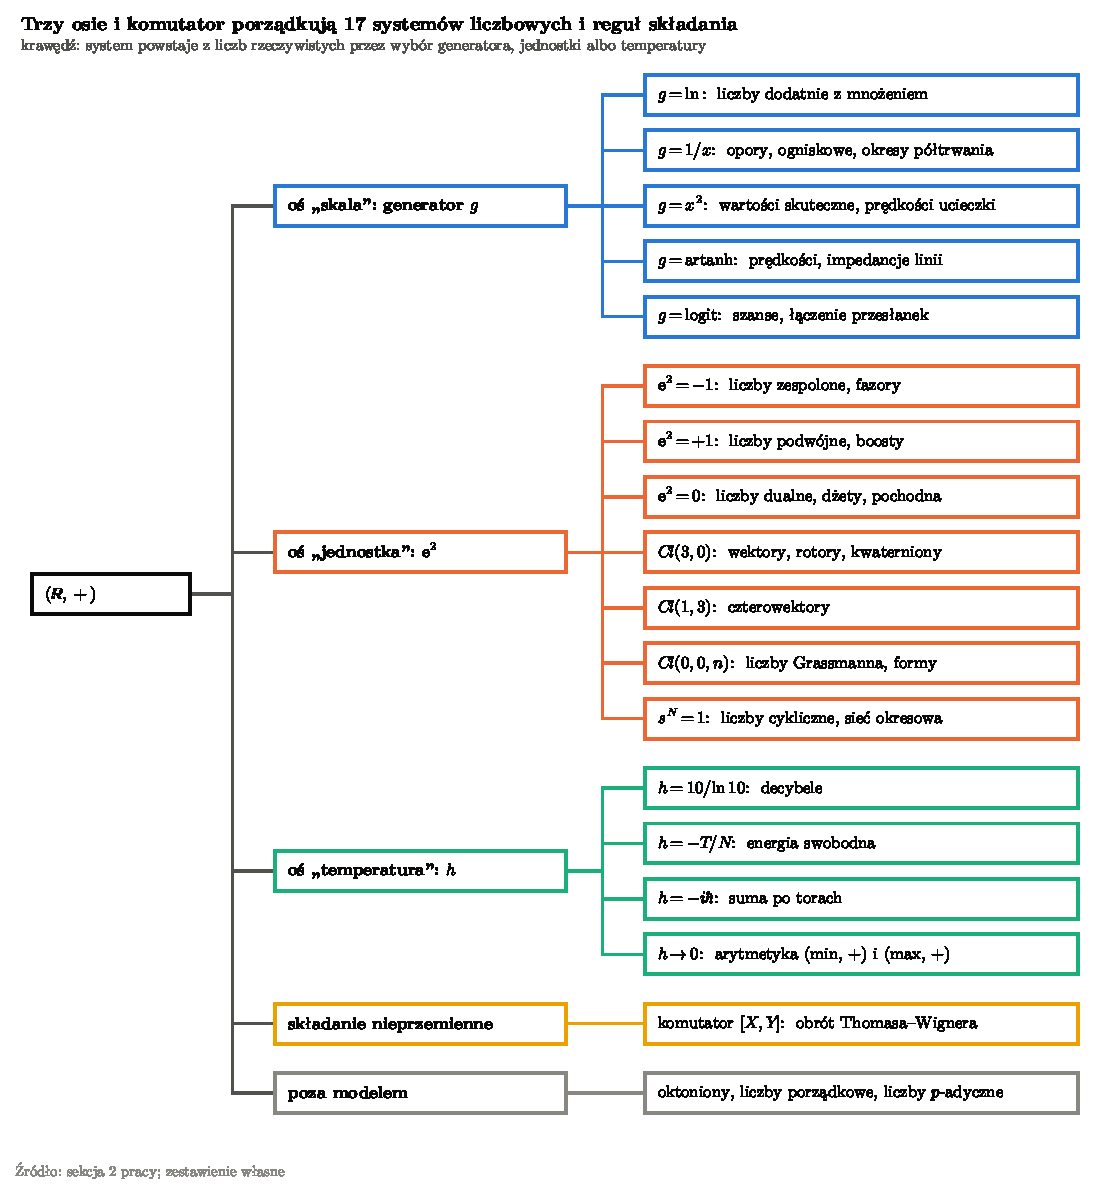
\includegraphics[width=0.8\textwidth]{figures/map.pdf}
\caption{Mapa systemów liczbowych. Każdy węzeł jest połączony z węzłem
$(\mathbb{R},+)$; krawędzie biegną tylko poziomo i pionowo.}
\label{fig:map}
\end{figure}

Funkcja pełni w modelu jedną z trzech ról.
\begin{enumerate}[label=(\alph*),leftmargin=2.2em]
  \item Generator. Każda funkcja ciągła i ściśle monotoniczna na przedziale
        zadaje skalę \cite{szulia2026}.
  \item Wykładnik jednostki. Funkcje $\cos$, $\sin$, $\cosh$, $\sinh$ oraz para
        $(1, t)$ to części funkcji $\exp(\ue t)$ ze wzoru \eqref{eq:exp}.
  \item Wzór na dodawanie. Jeżeli $f(x+y)=F\big(f(x),f(y)\big)$ i $f$ jest
        bijekcją, to $F$ jest działaniem \eqref{eq:base} z generatorem
        $g=f^{-1}$. Przykład: wzór na $\tanh(x+y)$ daje składanie prędkości.
\end{enumerate}
Model nie wskazuje, który generator opisuje dane zjawisko. Wybór generatora,
jednostki i temperatury jest wiedzą fizyczną, a nie wynikiem modelu.

\section{Metoda}
\label{sec:method}

\paragraph{Dobór problemów.}
Wybraliśmy 2 problemy z każdego z 10 działów fizyki. Kryterium wyboru miało
dwie części: problem ma rozwiązanie podręcznikowe i problem używa co najmniej
1 osi modelu. Wybór nie jest losowy. Wynik pomiaru opisuje te 20 problemów,
a nie całą fizykę.

\paragraph{Dwa zapisy.}
Zapis klasyczny używa wektorów, macierzy, funkcji rzeczywistych i rozróżnienia
przypadków. Zapis nowy używa generatora, jednostek i sumy $\oph$. Każdy zapis
zawiera wzory potrzebne do obliczenia wyniku. Zapis nie zawiera wyprowadzenia.

\paragraph{Licznik symboli.}
Licznik stosuje każdą z trzech reguł do obu zapisów.
\begin{itemize}[leftmargin=1.6em]
  \item Za 1 symbol liczymy polecenie, które oznacza funkcję, literę grecką,
        operator albo strukturę; przykłady: kreska ułamkowa, $\sin$, $\omega$,
        $\oplus$.
  \item Za 1 symbol liczymy literę, liczbę, operator i nawias.
  \item Za 0 symboli liczymy klamry, znak indeksu dolnego, odstępy i polecenia
        kroju pisma.
\end{itemize}
Licznik mierzy tylko długość. Licznik nie mierzy trudności zapisu ani
czasu nauki notacji.

\paragraph{Test zgodności.}
Dla każdego problemu kod oblicza wynik dwiema drogami i zapisuje odchyłkę.
W \gcTight{} problemach odchyłka nie przekracza $\gcResidMax$. Trzy problemy
mają większą tolerancję z podanego powodu.
\begin{itemize}[leftmargin=1.6em]
  \item Problem H, tolerancja $10^{-6}$: pola cyklu Carnota pochodzą
        z kwadratury na 8000 punktów.
  \item Problem N, tolerancja $10^{-3}$: arytmetyka $\lambda^{2}=0$ jest
        dokładna do pierwszego rzędu, a całkowanie orbity zawiera człony rzędu
        $\lambda^{2}$.
  \item Problem P, tolerancja $10^{-3}$: okno sumy po torach dodaje człon rzędu
        $\hbar/L^{2}$, gdzie $L$ to połowa szerokości okna.
\end{itemize}

\paragraph{Odtworzenie wyników.}
Trzy polecenia odtwarzają każdą liczbę i każdy rysunek pracy.
\begin{itemize}[leftmargin=1.6em]
  \item \texttt{python -m src.problems} wykonuje 20 testów i zapisuje wyniki.
  \item \texttt{python scripts/figures.py} rysuje 12 rysunków i 10 animacji.
  \item \texttt{python -m pytest -q} powtarza testy.
\end{itemize}

\section{Wyniki}
\label{sec:results}

\subsection{Zestawienie}

Tabela \ref{tab:results} i rysunek \ref{fig:lengths} podają wynik pomiaru.
Nowy zapis jest krótszy w \gcShorter{} problemach i dłuższy w \gcLonger{}
problemach. Suma długości 20 zapisów spada z \gcSumClassic{} do \gcSumNew{}
symboli. Mediana ilorazu długości wynosi \gcMedian. Iloraz najmniejszy to
\gcRatioMin{} (problem \gcRatioMinId), a iloraz największy to \gcRatioMax{}
(problem \gcRatioMaxId).

Zapis nowy jest dłuższy w problemach \gcLongerIds. W każdym z tych problemów
zapis klasyczny ma co najwyżej 4 wzory, a zapis nowy dodaje definicję skali
albo nowej zmiennej. Opisy tych problemów podają, co
zapis nowy daje w zamian.

\begin{table}[t]
\centering
\small
\caption{Dwadzieścia problemów. Kolumny: oś modelu, liczba symboli zapisu
klasycznego ($n_{k}$) i zapisu nowego ($n_{n}$), iloraz $n_{n}/n_{k}$ oraz
odchyłka testu zgodności. Plik źródłowy: \texttt{results\_problems.json}.}
\label{tab:results}
\begin{tabular}{@{}c l l r r r r@{}}
\toprule
& \textbf{problem} & \textbf{oś} & $n_{k}$ & $n_{n}$ & \textbf{iloraz} & \textbf{odchyłka} \\
\midrule
\gcRows
\bottomrule
\end{tabular}
\end{table}

\begin{figure}[t]
\centering
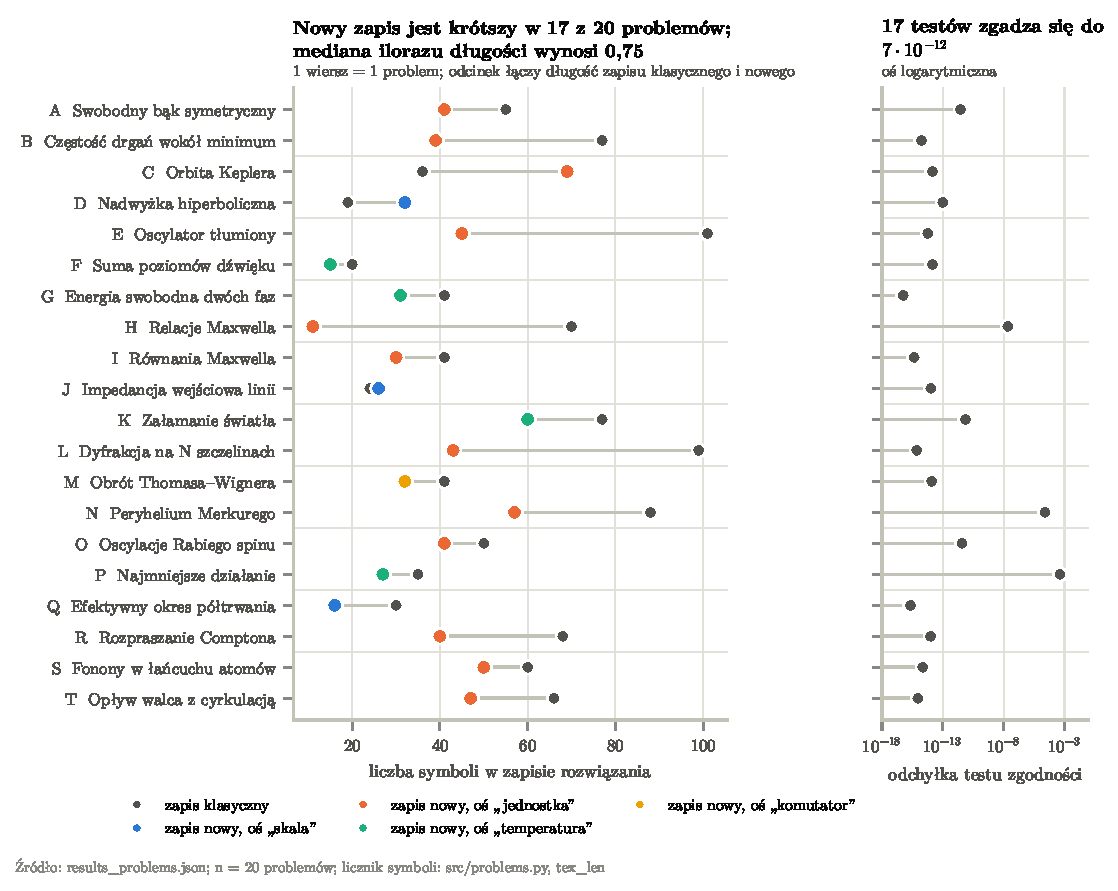
\includegraphics[width=\textwidth]{figures/lengths.pdf}
\caption{Długość zapisu i odchyłka testu dla 20 problemów. Kolor punktu
oznacza oś modelu. Poziome linie oddzielają działy fizyki.}
\label{fig:lengths}
\end{figure}

\subsection{Mechanika klasyczna}

\paragraph{Problem A: swobodny bąk symetryczny.}
Bąk ma momenty bezwładności $I_{1}=I_{2}\neq I_{3}$. Na bąk nie działa moment
sił. Zapis klasyczny używa kątów Eulera względem osi momentu pędu. Zapis nowy
używa rotora, czyli wykładnika jednostek o kwadracie $-1$.
\zapisy{A}
Symbol $\ps\mathbf{L}$ oznacza moment pędu jako wielowektor stopnia 2, a $R_{0}$
oznacza położenie początkowe. Położenie bąka w chwili $t$ to
$v\mapsto Rv\tilde{R}$. Test porównuje wzór z rotorem i całkowanie równań Eulera
metodą Rungego--Kutty rzędu 4 (RK4). Odchyłka wynosi \odchylka{A}.

\paragraph{Problem B: częstość drgań wokół minimum potencjału.}
Cząstka o masie $m$ drga wokół minimum $r_{0}$ potencjału Lennarda-Jonesa
$V(r)=4\epsilon\big((\sigma/r)^{12}-(\sigma/r)^{6}\big)$. Zapis klasyczny wymaga
dwóch pochodnych policzonych ręcznie. Zapis nowy podstawia do potencjału liczbę
$r_{0}+\varepsilon$ z regułą $\varepsilon^{3}=0$.
\zapisy{B}
Arytmetyka dżetów \eqref{eq:jet} daje $c_{2}=V''(r_{0})/2$ bez wzoru na
pochodną. Dla $\epsilon=\sigma=m=1$ wynik to $V''(r_{0})=\gcLJk$
i $\omega=\gcLJomega$. Odchyłka od wzoru $72\epsilon/(2^{1/3}\sigma^{2})$
wynosi \odchylka{B}. Iloraz różnicowy ma w tym samym zadaniu błąd względny
co najmniej $\gcLJfd$ (rysunek \ref{fig:b01}).

\rysunekdzialu{01}{}{Mechanika klasyczna. Panel lewy: problem A, składowe osi
symetrii bąka z rotora i z całkowania. Panel prawy: problem B, błąd drugiej
pochodnej potencjału.}

\subsection{Grawitacja i mechanika nieba}

\paragraph{Problem C: orbita Keplera.}
Ciało krąży po elipsie o półosi $a$ i mimośrodzie $e$ wokół masy o parametrze
grawitacyjnym $\mu$. Zapis klasyczny wymaga rozwiązania równania Keplera, które
jest przestępne względem anomalii $E$. Zapis nowy używa spinora Leviego-Civity
$w$ i czasu fikcyjnego $s$ z regułą $dt=|z|\,ds$ \cite{levicivita1920}.
\zapisy{C}
Liczba zespolona $z=x+iy$ to położenie ciała. Zapis nowy jest dłuższy.
W zamian równanie ruchu jest równaniem oscylatora harmonicznego: jest liniowe
i nie ma osobliwości w punkcie $z=0$. Test porównuje zapis nowy z całkowaniem
równania Newtona; odchyłka wynosi \odchylka{C}. Rysunek \ref{fig:b02} pokazuje
skutek liczbowy: przy mimośrodzie $0{,}9$ i 1000 kroków na okres błąd metody
RK4 w czasie $s$ jest mniejszy o \gcKeplerOrders{} rzędów wielkości.

\paragraph{Problem D: nadwyżka hiperboliczna.}
Sonda mija planetę po paraboli. W perycentrum $r_{p}$ silnik zwiększa prędkość
sondy o $\Delta v$. Szukamy prędkości $v_{\infty}$ daleko od planety. Zapis nowy
to odejmowanie w skali $g(v)=v^{2}$ z pierwszej pracy.
\zapisy{D}
Zapis nowy jest dłuższy, bo wymaga definicji prędkości ucieczki $v_{e}$.
W zamian zapis nowy niesie informację o strukturze. Arytmetyka potęgowa jest
monoidem \cite{szulia2026}: różnica $a\gsub b$ istnieje tylko dla $a\ge b$.
Warunek istnienia różnicy jest warunkiem orbity otwartej. Impuls
$\Delta v=0{,}1\,v_{e}$ daje $v_{\infty}=\gcOberth\,v_{e}$. Zysk rośnie, gdy
zapłon następuje bliżej planety. Odchyłka testu wynosi \odchylka{D}.

\rysunekdzialu{02}{}{Grawitacja i mechanika nieba. Panel lewy: problem C, błąd
położenia po 1 okresie dla dwóch zmiennych niezależnych. Panel prawy:
problem D, prędkość końcowa po impulsie w odległości $r$.}

\subsection{Drgania, fale i akustyka}

\paragraph{Problem E: oscylator tłumiony.}
Oscylator spełnia równanie $\ddot{x}+2\gamma\dot{x}+\omega_{0}^{2}x=0$
z warunkami $x(0)=x_{0}$ i $\dot{x}(0)=v_{0}$. Zapis klasyczny ma trzy
przypadki. Zapis nowy ma jeden wzór z jednostką $\ue$ o kwadracie
$\gamma^{2}-\omega_{0}^{2}$.
\zapisy{E}
Funkcje $C$ i $S$ pochodzą ze wzoru \eqref{eq:exp}. Tłumienie krytyczne to
przypadek liczb dualnych: $\ue^{2}=0$, $C=1$, $S=t$. Odchyłka od całkowania
RK4 w trzech przypadkach wynosi \odchylka{E}.

\paragraph{Problem F: suma poziomów dźwięku.}
Dwa niespójne źródła dźwięku mają poziomy $L_{1}$ i $L_{2}$ w decybelach. Zapis
nowy to suma z temperaturą $h=10/\ln10=\gcDbH$ dB.
\zapisy{F}
Gdy różnica $L_{1}-L_{2}$ rośnie, suma dąży do $\max(L_{1},L_{2})$
(stwierdzenie \ref{prop:limit}). Dwa źródła po 80 dB dają
\gcDbSame{} dB. Źródło słabsze o 10 dB dodaje \gcDbTen{} dB. Odchyłka testu
wynosi \odchylka{F}.

\rysunekdzialu{03}{}{Drgania, fale i akustyka. Panel lewy: trzy rodzaje
jednostek we wzorze \eqref{eq:exp}. Panel prawy: problem F, dodatek do
głośniejszego źródła.}

\subsection{Termodynamika i fizyka statystyczna}

\paragraph{Problem G: energia swobodna dwóch faz.}
Układ $N$ cząstek ma dwie fazy. Energia swobodna na cząstkę wynosi $f_{1}$
w fazie pierwszej i $f_{2}$ w fazie drugiej. Temperatura układu to $T$,
a stała Boltzmanna wynosi 1.
\zapisy{G}
Granica termodynamiczna $N\to\infty$ jest granicą $h\to0^{-}$. Przejście fazowe
pierwszego rodzaju to załamanie funkcji $\min(f_{1},f_{2})$. Dla skończonego
$N$ załamanie jest wygładzone, a różnica nie przekracza $(T/N)\ln2$
(stwierdzenie \ref{prop:limit}). Ta sama suma daje ciepło właściwe układu
dwupoziomowego o przerwie $\Delta$: dżet rzędu 2 liczy drugą pochodną energii
swobodnej. Maksimum ciepła właściwego wynosi \gcSchottkyC{} $k_{B}$ przy
$k_{B}T=\gcSchottkyT\,\Delta$. Odchyłka testu wynosi \odchylka{G}.

\paragraph{Problem H: relacje Maxwella.}
Cztery relacje Maxwella wiążą pochodne temperatury $T$, entropii $S$, ciśnienia
$p$ i objętości $V$. Zapis nowy to jedna tożsamość dla różniczek, które są
jednostkami o kwadracie $0$ w algebrze $Cl(0,0,2)$.
\zapisy{H}
Wybór pary zmiennych niezależnych, kolejno $(S,V)$, $(S,p)$, $(T,V)$ i $(T,p)$,
daje cztery relacje klasyczne. Test liczy współczynnik iloczynu
$dT\wedge dS-dp\wedge dV$ dla gazu van der Waalsa i dla gazu doskonałego. Test
porównuje też pola cyklu Carnota w płaszczyznach $(V,p)$ i $(S,T)$; oba pola
wynoszą \gcCarnotArea. Odchyłka testu wynosi \odchylka{H}.

\rysunekdzialu{04}{}{Termodynamika i fizyka statystyczna. Panel lewy:
problem G, ciepło właściwe układu dwupoziomowego. Panel prawy: problem H,
cykl Carnota w dwóch płaszczyznach.}

\subsection{Elektryczność i magnetyzm}

\paragraph{Problem I: równania Maxwella.}
Zapis klasyczny ma cztery równania dla pól $\mathbf{E}$ i $\mathbf{B}$. Zapis
nowy ma jedno równanie dla wielowektora $F$ w algebrze $Cl(3,0)$.
\zapisy{I}
Części równania o stopniach 0, 1, 2 i 3 to kolejno: prawo Gaussa, prawo
Ampère'a--Maxwella, prawo Faradaya i brak ładunków magnetycznych. Test liczy
8 składowych obu zapisów w 40 punktach dla pola, które nie spełnia równań.
Pochodne pola pochodzą z dżetów. Odchyłka wynosi \odchylka{I}.

\paragraph{Problem J: impedancja wejściowa linii.}
Linia bezstratna ma impedancję falową $Z_{0}$, stałą fazową $\beta$ i długość
$l$. Linię zamyka obciążenie $Z_{L}$. Zapis nowy mówi, że w skali
$g=\artanh$ odcinek linii dodaje liczbę $j\beta l$.
\zapisy{J}
Zapis nowy jest dłuższy o 2 symbole. W zamian zapis nowy pokazuje wspólną
strukturę: ten sam generator składa prędkości w szczególnej teorii względności
\cite{szulia2026}. Dwa odcinki linii dodają długości elektryczne. Odcinek
ćwierćfalowy dodaje $j\pi/2$, co zamienia $z$ na $1/z$. Odchyłka testu wynosi
\odchylka{J}.

\rysunekdzialu{05}{}{Elektryczność i magnetyzm. Panel lewy: problem I,
składowe czterech równań i jednego równania. Panel prawy: problem J,
współczynnik odbicia wzdłuż linii.}

\subsection{Optyka}

\paragraph{Problem K: załamanie światła.}
Światło biegnie z punktu A w ośrodku o współczynniku $n_{1}$ do punktu B
w ośrodku o współczynniku $n_{2}$. Punkt A leży w odległości $a$ od granicy
ośrodków, punkt B w odległości $b$, a odstęp punktów wzdłuż granicy wynosi $d$.
Zapis klasyczny to prawo Snella i geometria; położenie $x$ punktu przejścia
spełnia równanie stopnia 4.
\zapisy{K}
Zapis nowy to iloczyn dwóch macierzy w arytmetyce $(\min,+)$: czas dojścia jest
sumą $\oplus$ po punktach granicy. Prawo Snella wynika z minimum i nie wchodzi
do zapisu. Odchyłka czasu wynosi \odchylka{K}. Na siatce 200\,001 punktów
granicy różnica $|n_{1}\sin\theta_{1}-n_{2}\sin\theta_{2}|$ wynosi
$\gcSnellDefect$.

\paragraph{Problem L: dyfrakcja na $N$ szczelinach.}
Fala płaska pada na $N$ szczelin. Różnica faz sąsiednich szczelin wynosi
$\delta$. Zapis klasyczny bez liczb zespolonych sumuje osobno cosinusy
i sinusy. Zapis nowy sumuje szereg geometryczny fazorów.
\zapisy{L}
Odchyłka testu wynosi \odchylka{L}.

\rysunekdzialu{06}{}{Optyka. Panel lewy: problem K, prawo Snella w punkcie
minimum dla 60 geometrii. Panel prawy: problem L, natężenie dla 2, 5
i 10 szczelin.}

\subsection{Teoria względności}

\paragraph{Problem M: obrót Thomasa--Wignera.}
Dwa boosty mają pospieszności $\eta_{1}$ i $\eta_{2}$ oraz kierunki
$\mathbf{n}_{1}$ i $\mathbf{n}_{2}$ pod kątem $\alpha$. Złożenie dwóch boostów
to boost $B$ i obrót $R$ o kąt $\theta$ \cite{thomas1926,wigner1939}. Zapis
klasyczny podaje gotowy wzór na kąt. Zapis nowy to iloczyn dwóch wykładników.
\zapisy{M}
Wektory przestrzeni mają w algebrze $Cl(3,0)$ kwadrat $+1$, więc boost to
$\exp(\eta\mathbf{n}/2)$. Pospieszności nie dodają się. Pierwszą poprawką we
wzorze \eqref{eq:bch} jest komutator, który jest generatorem obrotu. Dla
$\eta_{1}=\eta_{2}=0{,}1$ i $\alpha=90^{\circ}$ iloraz kąta dokładnego i kąta
z komutatora wynosi \gcWignerSmall. Dwa prostopadłe boosty o prędkości
$0{,}9c$ obracają układ o $\gcWignerDeg^{\circ}$. Test porównuje iloczyn
wykładników, macierze $4\times4$ i wzór klasyczny; odchyłka wynosi
\odchylka{M}.

\paragraph{Problem N: peryhelium Merkurego.}
Ogólna teoria względności dodaje do równania orbity człon $3\mu u^{2}/c^{2}$,
gdzie $u=1/r$, a $h$ oznacza moment pędu na jednostkę masy
\cite{einstein1915}. Zapis klasyczny to rachunek zaburzeń z członem, który
rośnie z kątem $\varphi$. Zapis nowy traktuje parametr $\lambda$ jako jednostkę
o kwadracie $0$.
\zapisy{N}
W zapisie nowym $u_{0}$ to orbita kołowa w jednostkach $\mu/h^{2}$, a $\Omega$
to częstość drgań radialnych. Obie wielkości są liczbami dualnymi. Dla
Merkurego $\lambda=\gcMercuryLambda\cdot10^{-8}$, a obrót peryhelium wynosi
$\gcMercuryArcsec''$ na stulecie. Dane orbity pochodzą z \cite{nasamercury},
a parametr grawitacyjny Słońca z \cite{prsa2016}. Test całkuje orbitę dla
$\lambda=10^{-5}$; odchyłka względna \odchylka{N} jest rzędu $\lambda$.

\rysunekdzialu{07}{}{Teoria względności. Panel lewy: problem M, kąt obrotu
dla dwóch prostopadłych boostów. Panel prawy: problem N, obrót peryhelium
w funkcji parametru $\lambda$.}

\subsection{Mechanika kwantowa}

\paragraph{Problem O: oscylacje Rabiego spinu.}
Spin $1/2$ znajduje się w polu wirującym. W układzie wirującym pole ma częstość
Rabiego $\Omega_{R}$ i odstrojenie $\Delta$. Szukamy prawdopodobieństwa $P$
odwrócenia spinu \cite{rabi1937}. Zapis klasyczny to równanie Schrödingera
z macierzą $2\times2$. Zapis nowy używa tego samego rotora, który obraca bąk
w problemie A.
\zapisy{O}
Wektor spinu $\mathbf{s}$ obraca się wokół osi $\Omega_{R}e_{1}+\Delta e_{3}$.
Test porównuje rotor, całkowanie równania Schrödingera i wzór Rabiego; odchyłka
wynosi \odchylka{O}.

\paragraph{Problem P: najmniejsze działanie.}
Cząstka swobodna o masie $m$ przechodzi z punktu $0$ do punktu $X$ w czasie
$T$. Zapis klasyczny to równanie Eulera--Lagrange'a i działanie toru
klasycznego. Zapis nowy mówi, że działanie klasyczne jest granicą sumy $\oph$
po torach z temperaturą urojoną $h=-i\hbar$ \cite{feynman1948}.
\zapisy{P}
Test używa torów łamanych, które w połowie czasu przechodzą przez punkt $x$.
Działanie takiego toru to $S(x)=S+a(x-X/2)^{2}$, gdzie $a=2m/T$. Suma po torach
spełnia $h\ln\sum_{x}e^{S(x)/h}=S+\hbar\pi/4-(i\hbar/2)\ln(\pi\hbar/a)$.
Dwa człony z $\hbar$ znikają w granicy. Odchyłka sumy liczbowej od tego wzoru
wynosi \odchylka{P}. Ta sama suma z rzeczywistym $h$ opisuje decybele
(problem F) i energię swobodną (problem G).

\rysunekdzialu{08}{}{Mechanika kwantowa. Panel lewy: problem O, krzywe
Rabiego dla trzech odstrojeń. Panel prawy: problem P, moduł sumy po torach
w funkcji $\hbar$.}

\subsection{Fizyka atomowa, jądrowa i cząstek}

\paragraph{Problem Q: efektywny okres półtrwania.}
Izotop znika z organizmu dwoma kanałami: przez rozpad o okresie półtrwania
$T_{1}$ i przez wydalanie o okresie $T_{2}$. Zapis nowy to suma harmoniczna
z pierwszej pracy.
\zapisy{Q}
Dla wartości przykładowych $T_{1}=8$ d i $T_{2}=80$ d efektywny okres
półtrwania wynosi \gcHalfEff{} d. Test całkuje równanie rozpadu z dwoma
kanałami; odchyłka wynosi \odchylka{Q}.

\paragraph{Problem R: rozpraszanie Comptona.}
Foton o energii $E$ rozprasza się pod kątem $\theta$ na elektronie w spoczynku
\cite{compton1923}. Zapis klasyczny to trzy równania zachowania i eliminacja
pędu $p$ oraz kąta $\phi$ elektronu. Zapis nowy to kwadrat czterowektora
w algebrze $Cl(1,3)$ i suma harmoniczna energii.
\zapisy{R}
W zapisie nowym $p$, $k$ i $k'$ to czterowektory elektronu przed zderzeniem,
fotonu przed zderzeniem i fotonu po zderzeniu. W skali $g(x)=1/x$ wzór
Comptona jest linią prostą (rysunek \ref{fig:b09}). Odchyłka testu wynosi
\odchylka{R}.

\rysunekdzialu{09}{}{Fizyka atomowa, jądrowa i cząstek. Panel lewy:
problem Q, zanik liczby jąder dla 1 kanału i dla 2 kanałów. Panel prawy:
problem R, odwrotność energii fotonu rozproszonego.}

\subsection{Materia skondensowana i płyny}

\paragraph{Problem S: fonony w łańcuchu atomów.}
Pierścień $N$ atomów o masie $m$ łączą sprężyny o stałej $K$. Zapis klasyczny
to równanie ruchu, fala próbna i warunek okresowości \cite{kittel2005}. Zapis
nowy mówi, że macierz dynamiczna jest liczbą cykliczną $D$.
\zapisy{S}
Widmo macierzy to wartości liczby $D$ w pierwiastkach stopnia $N$ z jedności.
Test porównuje te wartości z wartościami własnymi macierzy $N\times N$ dla
$N=5$, $12$ i $64$; odchyłka wynosi \odchylka{S}.

\paragraph{Problem T: opływ walca z cyrkulacją.}
Płyn idealny opływa walec o promieniu $a$ z prędkością $U$ i cyrkulacją
$\Gamma$. Gęstość płynu wynosi $\rho$. Szukamy siły nośnej $Y$ na jednostkę
długości walca \cite{batchelor1967}. Zapis klasyczny to potencjał rzeczywisty,
ciśnienie z równania Bernoulliego i całka po powierzchni. Zapis nowy to
potencjał zespolony $w(z)$ i wzór Blasiusa.
\zapisy{T}
Siła jest w zapisie nowym residuum funkcji $(dw/dz)^{2}$. Test całkuje
ciśnienie po powierzchni walca i liczy całkę Blasiusa po okręgu; odchyłka
wynosi \odchylka{T}.

\rysunekdzialu{10}{}{Materia skondensowana i płyny. Panel lewy: problem S,
widmo łańcucha dla trzech długości. Panel prawy: problem T, ciśnienie na
powierzchni walca dla trzech wartości cyrkulacji.}

\FloatBarrier
\section{Zastosowania}
\label{sec:applications}

Każda oś modelu ma zastosowania, które działają w praktyce. Lista podaje
przykłady i nie jest pełna.

\paragraph{Skala.}
\begin{itemize}[leftmargin=1.6em]
  \item Obliczenia inżynierskie: opór zastępczy, ogniskowa układu soczewek,
        wartość skuteczna, poziom dźwięku \cite{szulia2026}.
  \item Technika mikrofalowa: wykres Smitha jest obrazem skali $\artanh$
        z problemu J \cite{pozar2012}.
  \item Statystyka: łączenie niezależnych przesłanek w skali logitu
        \cite{szulia2026}.
\end{itemize}

\paragraph{Jednostka.}
\begin{itemize}[leftmargin=1.6em]
  \item Grafika, robotyka i nawigacja: rotor opisuje orientację bez osobliwości
        kątów Eulera \cite{doran2003}.
  \item Uczenie maszynowe i optymalizacja: dżety są podstawą różniczkowania
        automatycznego \cite{griewank2008}.
  \item Mechanika nieba: zmienna $s$ z problemu C usuwa osobliwość zderzenia
        z równań ruchu \cite{levicivita1920}.
  \item Elektrotechnika i optyka: fazory zastępują sumy funkcji
        trygonometrycznych.
  \item Fizyka kryształów: liczby cykliczne dają widmo układu okresowego bez
        diagonalizacji macierzy \cite{kittel2005}.
\end{itemize}

\paragraph{Temperatura.}
\begin{itemize}[leftmargin=1.6em]
  \item Uczenie maszynowe: funkcja softmax i funkcja log-sum-exp to suma
        $\oph$. Sieć z funkcją aktywacji ReLU jest funkcją wymierną
        w arytmetyce tropikalnej \cite{zhang2018}.
  \item Planowanie: algebra $(\max,+)$ opisuje rozkłady jazdy i linie
        produkcyjne \cite{baccelli1992}. Algebra $(\min,+)$ opisuje najkrótszą
        drogę w grafie.
  \item Optyka i sejsmika: czas pierwszego dojścia fali jest iloczynem
        macierzy w arytmetyce $(\min,+)$ (problem K).
\end{itemize}

\paragraph{Nauczanie i oprogramowanie.}
Trzy osie dają jeden słownik pojęć dla 10 działów fizyki. Ten sam rotor obraca
bąk (problem A) i spin (problem O). Ta sama suma $\oph$ opisuje decybele,
energię swobodną i sumę po torach. Plik \texttt{src/gcalc.py} realizuje trzy
osie i jest punktem wyjścia dla biblioteki typów liczbowych.

\section{Granice modelu}
\label{sec:limits}

\subsection{Co zostaje poza modelem}

\begin{itemize}[leftmargin=1.6em]
  \item \textbf{Oktoniony.} Mnożenie oktonionów nie jest łączne. Algebry
        Clifforda są łączne, więc model nie obejmuje oktonionów.
  \item \textbf{Liczby porządkowe.} Dodawanie liczb porządkowych nie jest
        przemienne i nie jest skracalne: $1+\omega=0+\omega$.
  \item \textbf{Liczby $p$-adyczne.} Zbiór liczb $p$-adycznych nie jest
        przedziałem prostej rzeczywistej, więc twierdzenie \ref{thm:aczel} go
        nie dotyczy.
  \item \textbf{Operator synergiczny.} Operator z pierwszej pracy nie jest
        łączny \cite{szulia2026}; model go nie obejmuje.
\end{itemize}

\subsection{Twierdzenia, których model nie uzasadnia}

\begin{enumerate}[leftmargin=1.6em]
  \item \textbf{Model opisuje świat lepiej niż matematyka dotychczasowa.}
        Model nie daje żadnego nowego przewidywania. Każdy wynik liczbowy
        w pracy jest znany. Model zmienia tylko zapis.
  \item \textbf{Nowy zapis jest zawsze krótszy.} Fałsz: zapis jest dłuższy
        w problemach \gcLongerIds.
  \item \textbf{Wynik dla 20 problemów opisuje całą fizykę.} Wybraliśmy
        problemy, które używają osi modelu. Próba nie jest losowa.
  \item \textbf{Krótszy zapis jest łatwiejszy.} Licznik symboli nie mierzy
        trudności. Czytelnik zapisu nowego ma do opanowania generator,
        jednostki i sumę $\oph$.
  \item \textbf{Model obejmuje każdy rodzaj liczb.} Fałsz: patrz lista
        z poprzedniej podsekcji.
  \item \textbf{Granica $h\to0$ wyjaśnia mechanikę kwantową.} Granica jest
        znaną metodą fazy stacjonarnej. Zapis $h=-i\hbar$ nadaje tej metodzie
        nazwę i nie dodaje treści fizycznej.
  \item \textbf{Model wskazuje właściwy generator.} Model podaje język.
        Wybór generatora, jednostki i temperatury dla danego zjawiska pochodzi
        z fizyki.
\end{enumerate}

\subsection{Zagrożenia dla trafności pomiaru}

Pomiar długości ma trzy słabe miejsca. Pierwsze: problemy i oba zapisy wybrał
ten sam autor. Drugie: licznik symboli zależy od konwencji notacji; inna
konwencja zmieni wartości w tabeli \ref{tab:results}. Trzecie: licznik nie
dolicza kosztu definicji z sekcji \ref{sec:axes}, które czytelnik poznaje raz
dla 20 problemów. Niezależne powtórzenie pomiaru wymaga listy problemów
ustalonej przed zapisem rozwiązań.

\section{Wnioski}

Trzy osie porządkują systemy liczbowe, których używa fizyka. Skala wybiera
współrzędną, w której składanie jest dodawaniem. Jednostka wybiera geometrię:
obrót, przesunięcie albo boost. Temperatura łączy dodawanie z działaniami
$\max$ i $\min$. Komutator mierzy to, czego nie usuwa żaden wybór skali.

Pomiar na 20 problemach daje następujący wynik. Nowy zapis jest krótszy
w \gcShorter{} problemach, a mediana ilorazu długości wynosi \gcMedian.
Największy zysk dają problemy, w których zapis klasyczny rozróżnia przypadki
albo wylicza składowe. Trzy problemy mają zapis dłuższy.

Dalsza praca ma trzy kierunki. Pierwszy: lista problemów ustalona z góry
i licznik oparty na gramatyce formalnej. Drugi: wersja angielska pracy. Trzeci:
porównanie na danych pomiarowych, które zapowiedziała pierwsza praca
\cite{szulia2026}.

{\footnotesize
\setlength{\itemsep}{1pt}
\begin{thebibliography}{99}
\bibitem{szulia2026} M. Szulia.
\emph{Arytmetyki generowane funkcją. Katalog, klasyfikacja strukturalna
i granice numeryczne schematu $a\oplus b=g^{-1}(g(a)+g(b))$}. 2026.
\url{https://github.com/maciejszulia/function-generated-arithmetics}
\bibitem{grossman1972} M. Grossman, R. Katz.
\emph{Non-Newtonian Calculus}. Lee Press, Pigeon Cove, 1972.
\bibitem{aczel1966} J. Aczél.
\emph{Lectures on Functional Equations and Their Applications}.
Academic Press, New York, 1966.
\bibitem{craigen1989} R. Craigen, Z. Páles.
The associativity equation revisited.
\emph{Aequationes Math.} 37 (1989), 306--312.
\bibitem{clifford1878} W. K. Clifford.
Applications of Grassmann's extensive algebra.
\emph{Amer. J. Math.} 1 (1878), 350--358.
\bibitem{yaglom1979} I. M. Yaglom.
\emph{A Simple Non-Euclidean Geometry and Its Physical Basis}.
Springer, New York, 1979.
\bibitem{hestenes2003} D. Hestenes.
Oersted Medal Lecture 2002: Reforming the mathematical language of physics.
\emph{Am. J. Phys.} 71 (2003), 104--121.
\bibitem{doran2003} C. Doran, A. Lasenby.
\emph{Geometric Algebra for Physicists}. Cambridge University Press, 2003.
\bibitem{griewank2008} A. Griewank, A. Walther.
\emph{Evaluating Derivatives: Principles and Techniques of Algorithmic
Differentiation}. Wyd. 2. SIAM, Philadelphia, 2008.
\bibitem{litvinov2007} G. L. Litvinov.
The Maslov dequantization, idempotent and tropical mathematics: a brief
introduction. \emph{J. Math. Sci.} 140 (2007), 426--444.
\bibitem{levicivita1920} T. Levi-Civita.
Sur la régularisation du problème des trois corps.
\emph{Acta Math.} 42 (1920), 99--144.
\bibitem{thomas1926} L. H. Thomas.
The motion of the spinning electron. \emph{Nature} 117 (1926), 514.
\bibitem{wigner1939} E. Wigner.
On unitary representations of the inhomogeneous Lorentz group.
\emph{Ann. Math.} 40 (1939), 149--204.
\bibitem{einstein1915} A. Einstein.
Erklärung der Perihelbewegung des Merkur aus der allgemeinen
Relativitätstheorie. \emph{Sitzungsber. Preuss. Akad. Wiss.} (1915), 831--839.
\bibitem{nasamercury} D. R. Williams.
\emph{Mercury Fact Sheet}. NASA Goddard Space Flight Center.
\url{https://nssdc.gsfc.nasa.gov/planetary/factsheet/mercuryfact.html}
\bibitem{prsa2016} A. Prša i in.
Nominal values for selected solar and planetary quantities: IAU 2015
Resolution B3. \emph{Astron. J.} 152 (2016), 41.
\bibitem{rabi1937} I. I. Rabi.
Space quantization in a gyrating magnetic field.
\emph{Phys. Rev.} 51 (1937), 652--654.
\bibitem{feynman1948} R. P. Feynman.
Space-time approach to non-relativistic quantum mechanics.
\emph{Rev. Mod. Phys.} 20 (1948), 367--387.
\bibitem{compton1923} A. H. Compton.
A quantum theory of the scattering of X-rays by light elements.
\emph{Phys. Rev.} 21 (1923), 483--502.
\bibitem{kittel2005} C. Kittel.
\emph{Introduction to Solid State Physics}. Wyd. 8. Wiley, 2005.
\bibitem{batchelor1967} G. K. Batchelor.
\emph{An Introduction to Fluid Dynamics}. Cambridge University Press, 1967.
\bibitem{pozar2012} D. M. Pozar.
\emph{Microwave Engineering}. Wyd. 4. Wiley, 2012.
\bibitem{zhang2018} L. Zhang, G. Naitzat, L.-H. Lim.
Tropical geometry of deep neural networks.
\emph{Proc. 35th Int. Conf. on Machine Learning}, PMLR 80 (2018), 5824--5832.
\bibitem{baccelli1992} F. Baccelli, G. Cohen, G. J. Olsder, J.-P. Quadrat.
\emph{Synchronization and Linearity: An Algebra for Discrete Event Systems}.
Wiley, 1992.
\end{thebibliography}
}

\end{document}
